% siminos/ksReduced/ksReduced.tex    pdflatex ksReduced
% $Author$ $Date$

% ES ver. 2.0 reboot: re-started writing 			2011-11-03
%   after being interrupted by job applications,
%   childbirth, moving to Dresden, real plumbing, etc.
% ES started writing and thinking sometime in		March 2011

                \newif\ifdraft \drafttrue
%\draftfalse     % For web and journal version, no comments
                \ifdraft
%% Use sparingly. Date your comment. Once settled,
%% please move to siminos/blog/freeze.tex (append at the end)
\newcommand{\PCedit}[1]{{\color{magenta}#1}}
\newcommand{\ESedit}[1]{{\color{blue}#1}}
\newcommand{\RLDedit}[1]{{\color{red}#1}}
\newcommand{\ES}[1]{\ESedit{\small [ES: #1]}}
\newcommand{\PC}[1]{\PCedit{\small[PC: #1]}}
\newcommand{\RLD}[1]{\RLDedit{\small [RLD: #1]}}
                \fi

% For chaos (see authors.aps.org/revtex4):
                \ifdraft
\documentclass[aip,cha,showpacs,reprint]{revtex4-1} % preprint
                \else
% change reprint -> preprint, remove twocolumn for journal submission
\documentclass[aip,cha,showpacs,twocolumn,
 		  reprint]{revtex4-1} % superscriptaddress, unsortedaddress
                \fi

\usepackage{amsmath,amsfonts,amssymb,amsbsy,amscd}
\usepackage[usenames,dvipsnames]{color}
\usepackage{hyperref}
\usepackage{graphicx}
\usepackage{ifthen}
\usepackage{color}

%%%%%%%%% Macros
%% ES: Please only add macros that will allow to easilly change journal.
%% Do not add macros to keep terminology, notation etc flexible.
%% Internal edits/comments macros are OK, as are some math macros already added.
%% PC: I feel personally persecuted. OK, OK, I surrender - you're the Boss.

\newcommand{\beq}{\begin{equation}}
\newcommand{\eeq}{\end{equation}}
\newcommand{\bseq}{\begin{subequations}}
\newcommand{\eseq}{\end{subequations}}
\newcommand{\barr}{\begin{array}}
\newcommand{\earr}{\end{array}}

\newcommand{\rf}     [1] {\cite{#1}}
\newcommand{\refref} [1] {Ref.~\onlinecite{#1}}
\newcommand{\refrefs}[1] {Refs.~\onlinecite{#1}}
\newcommand{\refeq}  [1] {(\ref{#1})}
\newcommand{\refeqs} [2]{(\ref{#1}--\ref{#2})}
\newcommand{\reffig} [1] {Fig.~\ref{#1}}
\newcommand{\refFig} [1] {Figure~\ref{#1}}
\newcommand{\refsect}[1] {Sect.~\ref{#1}}
\newcommand{\refappe}[1] {Appendix~\ref{#1}}
\newcommand{\reftab} [1] {Table~\ref{#1}}

\newcommand{\etc}{{etc.}}
\newcommand{\etal}{{\em et al.}}
\newcommand{\ie}{{i.e.}}
\newcommand{\cf}{{\em cf.\ }}
\newcommand{\eg}{{e.g.\ }}

\newcommand{\KS}{Kuramoto-Siva\-shin\-sky}
\newcommand{\KSe}{Kuramoto-Siva\-shin\-sky equation}
\newcommand{\pCf}{plane Couette flow}
\newcommand{\PCf}{Plane Couette flow}

\newcommand{\Rls}[1]{\ensuremath{\mathbb{R}^{#1}}}
\newcommand{\Clx}[1]{\ensuremath{\mathbb{C}^{#1}}}
\newcommand{\Un}[1]{\ensuremath{\textrm{U}(#1)}}         % in DasBuch
\newcommand{\On}[1]{\ensuremath{\textrm{O}(#1)}}
\newcommand{\SOn}[1]{\ensuremath{\textrm{SO}(#1)}}         % in DasBuch
\newcommand{\Dn}[1]{\ensuremath{\textrm{D}_{#1}}}              % in DasBuch
\newcommand{\Zn}[1]{\ensuremath{\textrm{C}_{#1}}}              % in DasBuch
\newcommand{\Ztwo}{\ensuremath{\textrm{C}_2}}                % in DasBuch
\newcommand{\Refl}{\ensuremath{\sigma}}

\newcommand{\chebT}{\mathrm{T}}
\newcommand{\chebU}{\mathrm{U}}

\newcommand{\Nd}{\ensuremath{d}} % state-space dimension
\newcommand{\Nc}{\ensuremath{N}} % complex state-space dimension

\newcommand{\ii}{\ensuremath{\mathrm{i}}} % \sqrt{-1}

%%%%%%% From chaosbook def.tex (copy them if absolutely necessary)
\newcommand{\wwwcb}[1]{       % keep homepage flexible:
                  {\tt \href{http://ChaosBook.org#1}
              {ChaosBook.org#1}}}
\newcommand{\arXiv}[1]{
              {\tt \href{http://arXiv.org/abs/#1}{arXiv:#1}}}
\newcommand{\weblink}[1]{{\tt \href{http://#1}{#1}}}
\newcommand{\jEigvec}[1][]{\ensuremath{{\bf e}^{(#1)}}} % right jacobiam eigenvector
\newcommand{\ExpaEig}{\ensuremath{\Lambda}}
\newcommand{\eigExp}[1][]{
\ifthenelse{\equal{#1}{}}{\ensuremath{\lambda}}{\ensuremath{\lambda^{(#1)}}}
                        }
\newcommand{\eigRe}[1][]{
\ifthenelse{\equal{#1}{}}{\ensuremath{\mu}}{\ensuremath{\mu^{(#1)}}}
                        }
\newcommand{\eigIm}[1][]{
  \ifthenelse{\equal{#1}{}}{\ensuremath{\omega}}{\ensuremath{\omega^{(#1)}}}
            }
\newcommand{\REQV}[2]{\ensuremath{TW_{#1#2}}} % #1 is + or -
\newcommand{\Poincare}{Poincar\'e}
 \newcommand{\EQV}[1]{\ensuremath{E_{#1}}}
\newcommand{\period}[1]{{\ensuremath{T_{#1}}}}
\newcommand{\Shift}{\ensuremath{\tau}}
\newcommand{\shift}{\ensuremath{d}}
\newcommand{\rpo}{rela\-ti\-ve periodic orbit}
\newcommand{\Rpo}{Rela\-ti\-ve periodic orbit}
\newcommand{\RPO}[1]{\ensuremath{\mathrm{RPO}_{#1}}}
% \newcommand{\RPO}[1]{\ensuremath{\text{RP$#1$}}}
% RPO_{period to 2-4 significant digits} - relative PO.  We use ^{+,-}
% to distinguish between members of a reflection-symmetric pair.

\newcommand{\ssp}{a}            % state space point
\newcommand{\vel}{\ensuremath{v}}   % state space velocity
\newcommand{\pSRed}{\ensuremath{\bar{\cal M}}} % reduced state space
\newcommand{\sspRed}{\ensuremath{\bar{\ssp}}}    % reduced state space point, experiment
\newcommand{\velRed}{\ensuremath{\bar{\vel}}}    % ES reduced state space velocity
\newcommand{\velRel}{\ensuremath{c}}    % relative state or phase velocity
\newcommand{\slicep}{\ensuremath{\bar{\ssp}'}}   % slice-fixing point, experimental
\newcommand{\timeAver} [1]{\overline{#1}}

%%%%%%% Setup hyperlinks
\definecolor{hreflinkcolor}{rgb}{0.13,0.17,0.83}
\hypersetup{colorlinks=true,urlcolor=hreflinkcolor,
		linkcolor=hreflinkcolor,citecolor=hreflinkcolor}
% Graphics files are in directory
\graphicspath{{../figs/}}
\bibliographystyle{plain}


\begin{document}

% ES: Please permute names as appropriate.
% PC: this order fine with me

\author{Evangelos Siminos}
\email{siminos@gatech.edu}
\affiliation{School of Physics,
	      Georgia Institute of Technology, Atlanta, GA 30332, USA}
% I find it fair to use GaTech affiliation here as this is
% improvement/continuation of the Thesis that Never Ends.
% PC: I'm glad you are using it.
\affiliation{Max Planck Institute for the Physics of Complex Systems,
N\"othnitzer Stra\ss e 38, D-01187 Dresden, Germany}

\author{Predrag Cvitanovi\'c}
\affiliation{School of Physics,
	      Georgia Institute of Technology, Atlanta, GA 30332, USA}

\author{Ruslan L. Davidchack}
\affiliation{Department of Mathematics,
	      University of Leicester, Leicester, LE1 7RH, UK}

\title{Freezing all waves: A global symmetry reduction of Kuramoto-Sivashinsky equation}
% previous titles:
% \title{Freezing of all waves: global symmetry reduction in Kuramoto-Sivashinsky equation}

\date{\today}

% no abstract used for CHAOS (?)
%%%%%%%%%%%%%%%%%%%%%%%%%%%%%%%%%%%%%%%%%%%%%%%%%%%%%%%%%%%%%%%%%%%%%%%%%%%%%%%%
%\begin{abstract}
%
%\end{abstract}
%%%%%%%%%%%%%%%%%%%%%%%%%%%%%%%%%%%%%%%%%%%%%%%%%%%%%%%%%%%%%%%%%%%%%%%%%%%%%%%%

            \pacs{
02.20.-a, 05.45.-a, 05.45.Jn, 47.27.ed
% 02.20.-a  Group theory, mathematics
% 05.45.-a 	Nonlinear dynamics and chaos
% 05.45.Jn 	High-dimensional chaos
% 47.10.Fg 	Dynamical systems methods (in Fluid Mechanics)
% 47.27.ed 	Dynamical systems approaches (turbulent flows)
% 47.52.+j 	Chaos in fluid dynamics
% 42.65.Sf 	Dynamics of nonlinear optical systems; optical instabilities,
% 		optical chaos and complexity, and optical spatio-temporal dynamics
            }

\maketitle

%%%%%%%%%%%%%%%%%%%%%%%%%%%%%%%%%%%%%%%%%%%%%%%%%%%%%%%%%%%%%%%%%%%%%%%%%%%%%%%%

% CHAOS requires a paragraph of text to precede the first \section of the
% article; this is known as a lead paragraph and is formatted boldface. To
% give your article a lead paragraph, include a quotation environment ahead
% of the first \section command
%%%%%%%%%%%%%%%%%%%%%%%%%%%%%%%%%%%%%%%%%%%%%%%%%%%%%%%%%%%%%%%%%%%%%%%%%%%%%%%%
\begin{quotation}
symmetry reduction

which yield {globally} well behaved
transformations to invariant variables

    \PC{2011-12-23
Date your comments. Once settled, please move them to
siminos/blog/freeze.tex (append at the end)
    }
\end{quotation}
%%%%%%%%%%%%%%%%%%%%%%%%%%%%%%%%%%%%%%%%%%%%%%%%%%%%%%%%%%%%%%%%%%%%%%%%%%%%%%%%

\section{Introduction\label{s:intro}}

% Recent developments in the study of fluids and other dissipative,
% spatially-extended systems suggest that certain types of intrinsically
% low-dimensional behavior can be understood by means of the theory of
% dynamical systems. In particular, studies of the Kuramoto-Sivashinsky
% partial differential equation (PDE) and of the plane Couette flow indicate that
% the low-dimensional manifolds of unstable equilibria play the key role in
% organizing the high-dimensional state-space, in a way familiar from the study
% of low-dimensional systems of ordinary differential equations (ODEs).
% An important limitation of studies that embrace this point of view is that,
% so far, the significance of traveling wave solutions as organizing centers
% has not been clarified, even though these constitute the most commonly
% encountered stationary solutions in fluid flows.
%
% Wave motion appears as a result of the translational symmetry of the partial
% differential equations that describe continuous media, which in turn can be
% traced back to the basic assumptions on the nature of space and the physical
% laws. Waves which maintain a constant shape during their propagation,
% also termed relative equilibria, are translationally invariant solutions and can
% be thought of as equilibria in a co-moving frame. However, we are interested here
% in a global state-space picture and, as multiple traveling waves of different
% speeds commonly exist for any given flow parameter, the use of a single
% co-moving frame is rendered problematic for our purposes. Moreover, solutions
% with broken symmetry also do exist, for instance modulated traveling waves in
% which the wave profile is characterized by a periodic modulation (whence the
% alternative name relative periodic orbit). Furthermore, the generic,
% turbulent solutions are characterized by drifts along the direction of wave
% propagation.
%
% To illustrate how this obscures the understanding of global
% state-space geometry, we present in \reffig{f:ksIntro}(a) a state-space
% portrait of the Kuramoto-Sivashinsky (KS) flow
% (introduced in \refsect{s:notions}), in a periodic spatial domain of length
% $L=22$. We think of the KS flow in terms of its $\Nd$-dimensional Fourier
% space truncation, with $\Nd$ large enough for well-resolved simulations.
% The projection in \reffig{f:ksIntro}(a) is onto the the real parts of
% the three leading Fourier modes and suffers from the tendency of solutions to drift
% around (in Fourier space, translations become rotations).
%
% The main achievement of this paper is to show how the mess
% of \reffig{f:ksIntro}(a) can be brought
% to the comprehensible and useful representation of \reffig{f:ksIntro}(b) in
% which the role of unstable manifolds of traveling waves in organizing the global
% geometry becomes apparent. The means by which the transition from
% \reffig{f:ksIntro}(a) to \reffig{f:ksIntro}(a) is achieved is \emph{symmetry
% reduction}: the variables onto which we project in \reffig{f:ksIntro}(b) are
% translationally invariant (or rotationally invariant if we think in terms of
% Fourier modes) and span the $\Nd-1$-dimensional \emph{reduced space} in which
% wave motion appears frozen.
%

The relation of such singularities to the choice of a slice has been
discussed in \refrefs{SiminosThesis,SiCvi10,FrCv11}. In
\refrefs{rowley_reconstruction_2000,SiCvi10,FrCv11} the use of multiple
local hyperplane slices to cover state space has been proposed. However,
the task of picking such a set of slices and piecing them together in a
manner that does not obscure the global picture appears highly non-trivial,
and we know of no successful implementation of such state-space tessellation
proposals. Here we will take a different path and introduce modifications
of equations \refeq{eq:O2cheb} which yield \emph{globally} well behaved
transformations to invariant variables.

Following \refref{SCD07}, all computations in this paper are carried out
for $L = 22$ system. For this system size Davidchack (unpublished) has
computed $\approx 60,000$ relative-periodic and pre-periodic orbits using
the numerical method described in the appendix of \refref{SCD07}. The
database of these solutions together with the corresponding Floquet
eigenvalues eigenvectors is available upon request.


\section{Basic notions\label{s:notions}}

the Kuramoto-Sivashinsky equation

evolution of $u=u(x,t)$ on a periodic domain $u(x,t) = u(x+L,t)$ is given
by
\beq
  u_t = F(u) = -{\textstyle\frac{1}{2}}(u^2)_x-u_{xx}-u_{xxxx}
    \,,\qquad   x \in [-L/2,L/2]
    \,.
\label{ks}
\eeq


In the Fourier representation
\beq
  u(x,t)=\sum_{k=-\infty}^{+\infty} a_k (t) e^{ i k x /\tilde{L} }
\,,
\label{eq:ksexp}
\eeq
where $ \tilde{L} = 2\pi/L$, the equation takes the form
\beq
\dot{a}_k= v_k(a)
     = ( q_k^2 - q_k^4 )\, a_k
    - i \frac{q_k}{2} \sum_{m=-\infty}^{+\infty} a_m a_{k-m}
\,,
\label{expan}
\eeq
where $q_k = k/\tilde{L}$. Since $u(x,t)$ is real, $a_k=a_{-k}^\ast$, and
we can replace the sum by a $k > 0$ sum.

It is convenient to represent complex modes as pairs of real variables,
either in cartesian or polar coordinates:
\[ a_k = (b_k, c_k) = b_k + ic_k = (r_k, \theta_k) = r_k e^{i\theta_k}
\,.
\]

$G$, the group of actions $ g \in G $ on a
state space (reflections, translations, \etc) is a symmetry of the KS
flow \refeq{ks} if $g\,u_t = F(g\,u)$.
The KS equation is time translationally invariant, and space translationally invariant
on a periodic domain under
the 1-parameter group of
$O(2): \{\Shift_{\shift/L},\Refl \}$.
If $u(x,t)$ is a solution, then
$\Shift_{\shift/L}\, u(x,t) = u(x+\shift,t)$
is an equivalent solution for any shift
$-L/2 < \shift \leq L/2$,
as is the
reflection (`parity' or `inversion')
\beq
    \Refl \, u(x) = -u(-x)
\,.
\label{KSparity}
\eeq
The translation operator action on the Fourier coefficients \refeq{eq:ksexp},
represented here by a complex valued vector
$a = \{a_k\in\mathbb{C}\,|\,k = 1, 2, \ldots\}$, is given by
\beq
  \Shift_{\shift/L}\, a = \mathbf{g}(\shift) \, a \,,
  \label{eq:shiftFour}
\eeq
where $\mathbf{g}(\shift) = \mbox{diag}( e^{i q_k\, \shift} )$ is a complex
valued diagonal matrix, which amounts to the $k$-th mode complex plane
rotation by an angle $k\, \shift /\tilde{L}$.  The reflection acts on
the Fourier coefficients by complex conjugation,
\beq
  \Refl \, a = -a^\ast
\,.
\label{FModInvSymm}
\eeq
Reflection generates the dihedral subgroup $D_1 = \{1, \Refl\}$
of $O(2)$.

\subsection{Relative periodic and pre-periodic orbits}
\label{s:rpoNumerics}

As a result of invariance under $\Shift_{\shift/L}$,
KS equation can have \rpo\ solutions
with a profile $u_p(x)$, period $\period{p}$, and a
nonzero shift $\shift_p$
\beq
  u(x+\shift_p,\period{p}) = u(x,0) = u_p(x)
\,.
\label{eq:KSrpos}
\eeq
{\Rpo s} are periodic in
co-rotating frame rotating with phase velocity
$\velRel_p=\shift_p/\period{p}$, but in the stationary frame
their trajectories are quasiperiodic.  Due to the reflection symmetry
\refeq{KSparity} of KS equation, every {\rpo} $u_p(x)$ with shift
$\shift_p$ has a symmetric partner $-u_p(-x)$ with shift $-\shift_p$.

\begin{table}[ht]
    \caption{
    Properties of equilibria and relative equilibria determining
    the system dynamics in their vicinity.  $T$ is characteristic
    time scale of the dynamics, $\ExpaEig_e$ and $\ExpaEig_c$ are the
    leading expansion and contraction multipliers, and $E$ is the
    energy \refeq{ksEnergy}.
            }
\begin{center} \footnotesize
    \begin{tabular}{l|rrrr}
                 & $E$~~   & $T$~~  & $\ExpaEig_e$  & $\ExpaEig_c$  \\ \hline
 $\EQV{1}\ $     &\ 0.2609 &\ 18.81 &\ 4.79     &\ 0.04 \\
 $\EQV{2}\ $     &\ 0.4382 &\ 26.35 &\ 5.99     &\ 0.03 \\
 $\EQV{3}\ $     &\ 1.5876 &\ 10.71 &\ 9.92     &\ 0.01 \\
 $\REQV{\pm}{1}$ &\ 0.4649 &  &  & \\
 $\REQV{\pm}{2}$ &\ 0.6048 &  &  & \\
    \end{tabular}
\end{center}
\label{tab:L22cminus}
\end{table}

%% A basic RevTeX table looks as follows:
%%  \begin{table}
%%  \caption{\label{tab:example}Text of table caption.}
\begin{table}
   \caption{\label{tab:RPOs}
      All rela\-ti\-ve equilib\-ria and some of the shortest \rpo s studied in this
      paper: rela\-ti\-ve equilib\-rium phase velocity $\velRel$ or \rpo\ mean phase velocity
      $\timeAver{\velRel}_p= \shift_p/\period{p}$; \rpo\ period
      $\period{p}$, shift $\shift_p$; (mean) dissipation $\timeAver{D}$;
      the number of unstable eigen-directions within the solution's
      symmetry subspace, $r= $~real, $c= $~complex (the numbers in
      brackets indicate the number of symmetry-breaking unstable
      eigenvalues when $\Omega_2$ is removed, with trailing $+$
      indicating that there may be more unstable eigenvalues, as only the
      largest few have been calculated so far); the leading  Floquet
      exponents $\eigExp[j]= \eigRe[j] \pm i\eigIm[j]$.
   }
   \centering
   \begin{tabular}{lclllllllll}
       & symm.           & $~~\timeAver{\velRel}$
                                   & ~~$\period{}$ &  ~~$\shift$
                                   & $\timeAver{D}$
                                   & \# unstable
                                   & $\eigRe[j]$ & $\eigIm[j]$
                                   \\
   \hline
   LB  &  $(S,\Omega_2)$  & 1.550 &&&& 1r (+0) \\ %1 & 0.0712 \\ % 1606
   ML  &  $(S,\Omega_2)$  & 1.421 &&&& 1c (+1r+2c) \\ %1 & 0.0224+0.0660i \\
   MU  &  $(S,\Omega_2)$  & 1.394 &&&& 1r (+1r+2c) \\ %1 & 0.0496 \\
   UB  &  $(S,\Omega_2)$  & 1.300 &&&& 3c (+3c+)  \\ %3 & 0.1517+1.7591i \\
   S2a &  $S$              & 1.304 &&&& 1c   \\ % 1856
   S2b &  $S$              & 1.522 &&&& 1r   \\ %1 & 0.0982 \\
   $\RPO{4.934}$ &  $(S,\Omega_2)$  & 1.369 & 4.934 &&& 1c (+4c+) \\ %244h
   $\RPO{10.96}$ &  $S$    & 1.302 & 10.96 &&& 1r+2c  \\ %2544
   $\RPO{36.72}$ &  $S$    & 2.178 & 36.72 &&& 1r+3c+  %2663
   \end{tabular}
\end{table}

A handful of the shortest \rpo s and pre-periodic orbits are listed in
    \reftab{tab:RPOs}.
For the lack of symbolic dynamics labeling of invariant solutions, we
refer to \rpo s as $\RPO{\period{}}$, labeled by the 3-4
significant digits of its period $\period{}$.
    \PC{2011-12-20 Either merge \reftab{tab:L22cminus} into
    \reftab{tab:RPOs}, or keep relative equilibria in
    \reftab{tab:L22cminus} only, harmonize the two tables. }

\section{From moving frames to invariant variables}

We begin by computing invariants for the ``standard action''
of $\SOn{2}$ on $\Clx{N}\cong\Rls{2N}$
which we write here as
% \beq
% 	\left(\barr{cc} \overline{b}_k \\ \overline{c}_k\earr \right)=\left(\barr{cc}
% 			    			\cos(k\theta) & -\sin(k\theta)\\
% 						\sin(k\theta) & \cos(k\theta)\\
% 			   			\earr	
% 						\right) \left(\barr{cc} b_k \\ c_k\earr\right)\,,\ \ k=1,\ldots N\,.
% 	\label{eq:SO2stand}
% \eeq
\bseq\label{eq:SO2stand}
  \begin{align}
	  \overline{b}_k &= \cos(k\theta)\,b_k - \sin(k\theta)\,c_k\,\label{eq:SO2stand1}\\
	  \overline{c}_k &= \sin(k\theta)\,b_k + \cos(k\theta)\,c_k\,,\label{eq:SO2stand2}
  \end{align}
\eseq
with $a_k=b_k+i c_k\,,\ b_k,c_k\in\Rls{}$ and $k=1,\ldots N$.
The choice of a slice is arbitrary; here we choose
\beq
 	\overline{c}_1=0\,,\qquad \overline{b}_1>0\,
\eeq
\RLD{If it's all the same to you, I'd suggest to set $\overline{b}_1=0$, which would be consistent with the definition of antisymmetric subspace we used before.}
\ES{It makes derivations (slightly) easier if I use this convention. I will keep it as it is and rethink at the end.}
which leads to
\beq
	\overline{c}_1 = b_1\,\sin\theta + c_1\,\cos\theta  = 0\,
	\label{eq:SO2norm}
\eeq
and the ``moving frame''
\beq
	\theta=-\tan^{-1}\frac{c_1}{b_1}\,.
	\label{eq:SO2mf}
\eeq
Here $\tan^{-1}$ distinguishes quadrants, so that our choice of a slice
results to
\beq\label{eq:phi1}
  \theta=-\phi_1\,,
\eeq
where $\phi_1$ the polar angle in the $a_1$ Fourier
subspace.


Pluging \refeq{eq:phi1} into \refeq{eq:SO2stand} and using
the identity
$\alpha\cos(\phi)+\beta\sin(\phi)=\sqrt{\alpha^2+\beta^2}\cos(\phi-\tan^{-1}(\beta/\alpha))$
we get
\bseq\label{eq:SO2polar}
  \begin{align}
    \overline{b}_k &=
		    r_k\, \cos(\phi_k-k\,\phi_1)\,, \label{eq:SO2polar1}\\
    \overline{c}_k &=
		    r_k\, \sin(\phi_k-k\,\phi_1)\,,\label{eq:SO2polar2}
  \end{align}
\eseq
for $k=1,\ldots N$, where $r_k\equiv\sqrt{b_i^2+c_i^2}$, and
$\phi_k$ the polar angle in the $a_k$ Fourier subspace.
Note that for $k=1$ we get $\overline{b}_1=r_1,\, \overline{c}_1=0$.
Thus we have arrived at a system of $2N-1$ variables, which according to
theorems of Fels and Olver\rf{FelsOlver98,FelsOlver99} are
$\SOn{2}$-invariant and functionally independent. They therefore serve the goal
of unique identification of group orbits, at least in the neighborhood of the
slice. We observe that \refeq{eq:SO2polar} are undefined at $r_1=0$,
a fact related to the familiar singularities of polar variables at the origin.
Tuckerman\rf{tuckerman89} showed that terms of the form $\psi_{n,k}(r,\phi)=r^n\exp(\ii\, k\,\phi)$
which appear in cylindrical coordinate $(r,\phi,z)$ discretizations of PDEs
are typically non-smooth at the origin. The problem is traced to rapid
oscillations of $\psi_{n,k}$ (with $\phi$) as $r\rightarrow0$ and Tuckerman\rf{tuckerman89} shows
that such oscillations are heavily damped near the origin for
$\psi_{n,k}$ with $n\geq k$. The prescription put forth by Tuckerman\rf{tuckerman89} to
construct a smooth basis for the numerical discretization of
PDEs is to keep only terms with $n\geq k$ (with some additional technical conditions).

The simplest way to modify variables \refeq{eq:SO2polar} to fulfill Tuckerman's
criterion is to multiply the right hand side by $r_1^k$. This would lead us to
work with invariant polynomials of order $k+1$ for the $k$'th Fourier subspace.
To see this, plug \refeq{eq:phi1} into \refeq{eq:SO2stand} to get
\bseq\label{eq:SO2cheb}
  \begin{align}
    \overline{b}_k &=
		    b_k\, \chebT_k\left(b_1/r_1\right)+
		    c_k\,\frac{c_1}{r_1} \chebU_{k-1}\left(b_1/r_1\right)\,, \label{eq:SO2cheb1}\\
    \overline{c}_k &=
		    b_k\, \frac{c_1}{r_1} \chebU_{k-1}\left(b_1/r_1\right)+
		    c_k\,\chebT_k\left(b_1/r_1\right)\,,  \label{eq:SO2cheb2}
  \end{align}
\eseq
where and $\chebT_k,\,\chebU_k$ are Chebyshev polynomials of the first and second type, respectively.
Therefore, multiplication by $r_1^k$ would result in highly deformed $a_k$ components
(and numerical underflow problems). Since our main goal is to investigate the
topology of the attractor we can instead aim at merely continuous or
differentiable transformations.
% Note also, that the introduction of a fundamental domain for discrete symmetry
% reduction destroys smoothness of the transformations, even if it is initially
% imposed in continuous symmetry reduction.

Thus, we multiply the right-hand side of \refeq{eq:SO2polar} with a monotonic function
$h_\epsilon(r_1)$ which satisfies $h_\epsilon(0)=0$,
has a convergent Maclaurin series for $0<r_1<\infty$,
and may depend on a parameter $\epsilon$.
Our modified set of $SO(2)$-invariants reads
\bseq\label{eq:SO2polarCont}
  \begin{align}
    \tilde{b}_k &=
		    h_\epsilon(r_1)\,\overline{b}_k\,, \label{eq:SO2polarCont1}\\
    \tilde{c}_k &=
		    h_\epsilon(r_1)\,\overline{c}_k\,, \quad k=1,\ldots,N.\label{eq:SO2polarCont2}
  \end{align}
\eseq
A simple choice for $h_\epsilon$ is
%are $h_\epsilon(r_1)=r_1$ which would lead to
%transformations \refeq{eq:SO2polarCont} continuous at $r_1=0$,
%and
$h_\epsilon(r_1)=r_1^2$ which would lead to differentiable transformations \refeq{eq:SO2polarCont}.
One can easily show that, with the above requirements,
\refeq{eq:SO2polarCont} are linearly independent. However,
\refeq{eq:SO2polarCont} maps any point in the subspace $r_1=0$ to zero, \ie\
\refeq{eq:SO2polarCont} do not provide a complete basis for the reduced space.
This a rather serious limitation, since non-trivial $N$-cell equilibria of
KSe are mapped to the origin under \refeq{eq:SO2polarCont}.

This difficulty suggests extending \refeq{eq:SO2polarCont} by including $2N-2$ additional linearly
independent invariant variables which do not vanish at $r_1=0$. To this end, we write
the transformations resulting from defining a slice $c_m=0,\, b_m>0$ for any $1<m\leq N$:
\bseq\label{eq:SO2polarAny}
  \begin{align}
    \overline{b}_k &=
		    r_k\, \cos\left(\phi_k-\left(k/m\right)\phi_m\right)\,, \label{eq:SO2polarAny1}\\
    \overline{c}_k &=
		    r_k\, \sin\left(\phi_k-\left(k/m\right)\phi_m\right)\,,\label{eq:SO2polarAny2}
  \end{align}
\eseq
for $k=1,\ldots N$. As before, we multiply variables \refeq{eq:SO2polarAny} by $h_\epsilon(r_m)$.
However, we have to note that only variables with $k=n\,m$, where $n$ integer, are well behaved.
Thus our basis reads
\bseq\label{eq:SO2polarExt}
\begin{align}
  \overline{b}_{nm} &=
		  h_\epsilon(r_m)r_{nm}\, \cos\left(\phi_{nm}-n\phi_m\right)\,, \label{eq:SO2polarAny1}\\
  \overline{c}_{nm} &=
		  h_\epsilon(r_m)r_{nm}\, \sin\left(\phi_{nm}-n\phi_m\right)\,,\label{eq:SO2polarAny2}
\end{align}
\eseq
$m=1,...,M$, $n=1,\ldots\lfloor N/m\rfloor$ and $M$ is the smallest integer that
satisfies $\sum_{m=2}^M(2\lfloor N/m\rfloor-1)\geq2N-2$ and for
$m=M$ we have $n=1,\ldots,\sum_{m=2}^M(2\lfloor N/m\rfloor-1)-(2N-2)$.

Variables \refeq{eq:SO2polarExt} are linearly, but not functionally independent. Therefore increase
in reduced space dimensionality is only apparent.
\ES{Here we could project back to $2N-1$ dimensions
through a linear transformation \emph{ala} Gilmore\rf{GL-Gil07b}. Another option is careful counting
of functional dependencies to figure out if we can simply pick $2N-1$ variables.}


% We can bypass this difficulty by adding an $r_k^2$ factor into the variables
% associated with the $k$'th Fourier subspace, in such a way that it respects
% reflection equivariance as expressed by \refeq{eq:SO2chebRefl}, to arrive to
% \bseq\label{eq:SO2inv}
%   \begin{align}
%     \tilde{b}'_k &=
% 		    r_1\,r_k\, \cos(\phi_k-k\,\phi_1)\,, \\
%     \tilde{c}'_k &=
% 		    r_k^2+r_1\,r_k\,\sin(\phi_k-k\,\phi_1)\,,
%   \end{align}
% for $k$ even, and
%   \begin{align}
%     \tilde{b}'_k &=
% 		    r_k^2+r_1\,r_k\, \cos(\phi_k-k\,\phi_1)\,, \\
%     \tilde{c}'_k &=
% 		    r_1\,r_k\, \cos(\phi_k-k\,\phi_1)\,,
%   \end{align}
% for $k$ odd.
% \eseq
% \bseq\label{eq:SO2polarContInd}
%   \begin{align}
%     \tilde{b}_k &=
% 		    \frac{1}{2}(1-(-1)^k)\,r_k^2+r_1\,\overline{b}_k\,, \label{eq:SO2polarCont1}\\
%     \tilde{c}_k &=
% 		    \frac{1}{2}(1-(-1)^{k+1})\,\,r_k^2+r_1\,\overline{c}_k\,.\label{eq:SO2polarCont2}
%   \end{align}
% \eseq

% Finally we need to factor out the discrete reflectional symmetry still present
% in \refeq{eq:SO2inv}. A simple but effective way to achieve this is
% by taking the absolute value of $\Refl$-equivariant variables
% in \refeq{eq:SO2inv}.
% As before, we factor out reflection symmetry by taking the absolute value
% of $\Refl$-equivariant variables in \refeq{eq:SO2inv}.
% Thus we are led to $\On{2}$-invariant variables
% \bseq\label{eq:O2inv}
%   \begin{align}
%     \beta_k &=
% 		    r_1\,r_k\, |\cos(\phi_k-k\,\phi_1)|\,, \\
%     \gamma_k &=
% 		    r_k^2+r_1\,r_k\,\sin(\phi_k-k\,\phi_1)\,,
%   \end{align}
% for $k$ even, and
%   \begin{align}
%     \beta_k &=
% 		    r_k^2+r_1\,r_k\, \cos(\phi_k-k\,\phi_1)\,, \\
%     \gamma_k &=
% 		    r_1\,r_k\, |\cos(\phi_k-k\,\phi_1)|\,,
%   \end{align}
% for $k$ odd.
% \eseq




 Under reflections $\Refl a_k \mapsto-b_k+\ii c_k$ we see that
\bseq\label{eq:SO2chebRefl}
 \begin{align}
  \overline{b}_k \mapsto (-1)^{k+1}\, \overline{b}_k\,,\\
  \overline{c}_k \mapsto (-1)^{k}\, \overline{c}_k\,.
 \end{align}
\eseq
%  To factor out the discrete reflection symmetry in \refeq{eq:SO2chebRefl} we can
% introduce a fundamental domain by taking the absolute value of those variables
% which are equivariant under $\Refl$, so that we are led to
% \bseq\label{eq:O2cheb}
%   \begin{align}
%     \overline{b}'_k &=
% 		    |\overline{b}_k|\,, \\
%     \overline{c}'_k &=
% 		    \overline{c}_k\,.
%   \end{align}
% for $k$ even, and
%   \begin{align}
%     \overline{b}'_k &=
% 		    \overline{b}_k\,, \\
%     \overline{c}'_k &=
% 		    |\overline{c}_k|\,.
%   \end{align}
% for $k$ odd.
% \eseq
%


% To shed more light into the origin of the singularities in \refeq{eq:O2cheb},
% we use the identity
% $\alpha\cos(\phi)+\beta\sin(\phi)=\sqrt{\alpha^2+\beta^2}\cos(x-\tan^{-1}(\beta/\alpha))$
% and plug \refeq{eq:phi1} into \refeq{eq:SO2stand}, to arrive to the
% ``polar'' form of \refeq{eq:SO2cheb}
% \bseq\label{eq:SO2polar}
%   \begin{align}
%     \overline{b}_k &=
% 		    r_k\, \cos(\phi_k-k\,\phi_1)\,, \label{eq:SO2polar1}\\
%     \overline{c}_k &=
% 		    r_k\, \sin(\phi_k-k\,\phi_1)\,,\label{eq:SO2polar2}
%   \end{align}
% \eseq
% where $\phi_k$ the polar angle in the $a_k$ Fourier subspace. In this coupled-polar
% % representation, it becomes apparent that the singularities of \refeq{eq:SO2cheb}
% are related to the familiar singularities of polar variables at the origin.
% Tuckerman\rf{tuckerman89} showed that terms of the form $\psi_{nk}(r,\phi)=r^n\exp(\ii\, k\,\phi)$
% which appear in cylindrical coordinate $(r,\phi,z)$ discretizations of PDEs
% are typically non-smooth at the origin. The problem is traced to rapid
% oscillations of $\psi_{nk}$ (with $\phi$) as $r\rightarrow0$ and Tuckerman\rf{tuckerman89} shows
% that such oscillations are heavily damped near the origin for
% $\psi_{nk}$ with $n\geq k$. The prescription put forth by Tuckerman\rf{tuckerman89} to
% construct a smooth basis for the numerical discretization of
% PDEs is to keep only terms with $n\geq k$
% (with some additional technical conditions).


\section{Symmetry reduced state space}


For all numerical results presented in this section we pick
$h_\epsilon(r_k)=(1-e^{-r_k^2/\epsilon})$ with $\epsilon=0.2$. This choice
scales as $r_k^2$ for $r_k\rightarrow 0$, thus ensuring differentiability
of \refeq{eq:SO2polarExt}, while for large $r_k$ distortion of
trajectories is minimal.

\begin{figure}
% ES used siminos/chao/matlab/ruslan/ks22reduced.m
 (a)~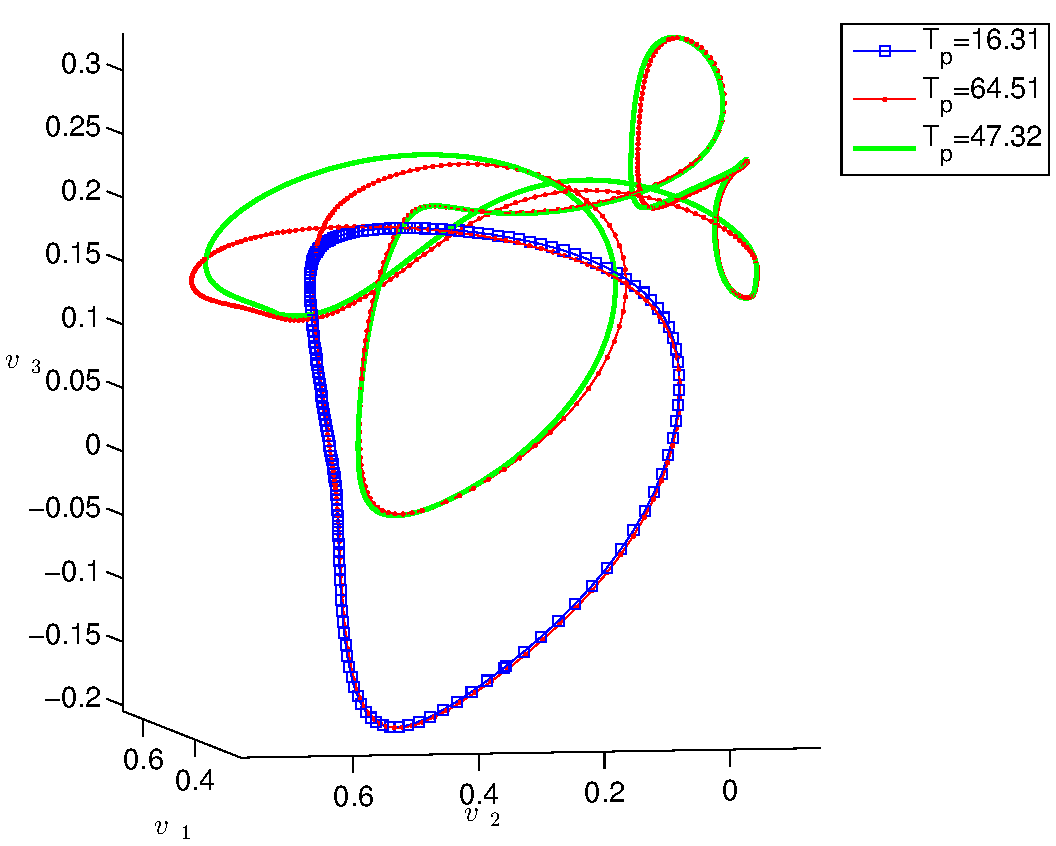
\includegraphics[width=0.40\textwidth]{ks22rpoT6451shad}
 (b)~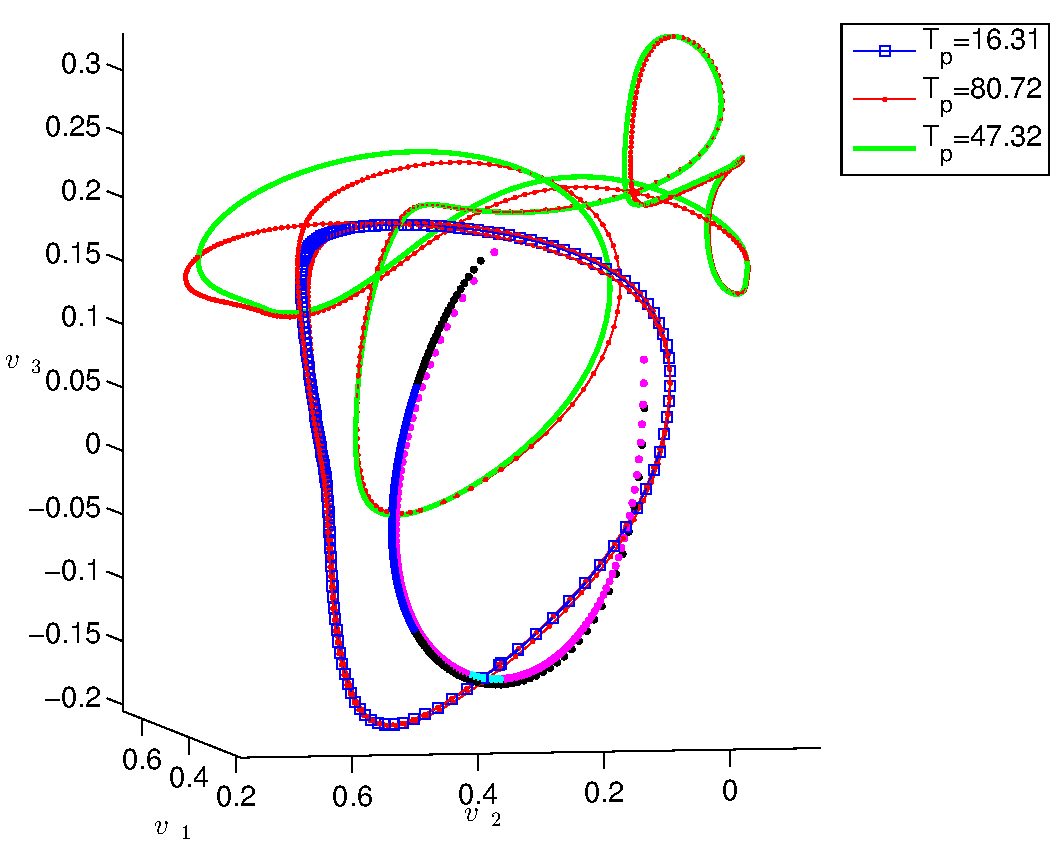
\includegraphics[width=0.40\textwidth]{ks22rpoT8072shad_manif}
\caption{
 Shadowing of \rpo s of \KSe\
% for $L=22.0$ (see \refref{SCD07}),
visualized in the invariant coordinate basis \refeq{eq:SO2polarExt}.
(a) \Rpo\ $\RPO{64.51}$ is shadowed by orbits $\RPO{16.32}$ and
$\RPO{47.32}$, (b) \Rpo\ $\RPO{80.71}$ is shadowed by orbits
$\RPO{16.32}$ and $\RPO{47.32}$. Note that $\RPO{80.71}$ traces
$\RPO{16.32}$ twice. Intersections of the unstable manifold of \rpo\
$\RPO{16.32}$ with a \Poincare\ section defined as a hyperplane
transverse to the flow at a state-space point $\ssp_{RPO{16.32}}(0)$ are
shown in cyan and magenta (first and second intersections, respectively).
Intersections of the unstable manifold of cycle $\RPO{47.32}$ with the
same \Poincare\ section are shown in blue and black (first and second
intersections, respectively). The coordinate axes $v_1$, $v_2$, and $v_3$
are constructed from Floquet eigenvectors $\jEigvec[1]$, $\jEigvec[4]$ on
\Poincare\ section fixing point $\ssp_{RPO{16.32}}(0)$, and unstable
eigenvector ${\Re\,} \jEigvec[1]$ of the relative equilibrium
\REQV{}{1}, by Gram-Schmidt orthogonalization in original space and
transformed to reduced space through transformations
\refeq{eq:SO2polarExt}.
}
\label{f:rpo_shad}
\end{figure}

    \ES{
In \refeq{f:rpo_shad} we can hope for some coarse symbolic dynamics
in which  $\RPO{64.51}$ is $01$ and $\RPO{80.71}$ is $001$. Return map
involving unstable manifolds of the two cycles is under construction, but
one can draw it mentally based on this figure already.
    }

\begin{figure*}[ht]
 \begin{center}
  (a)~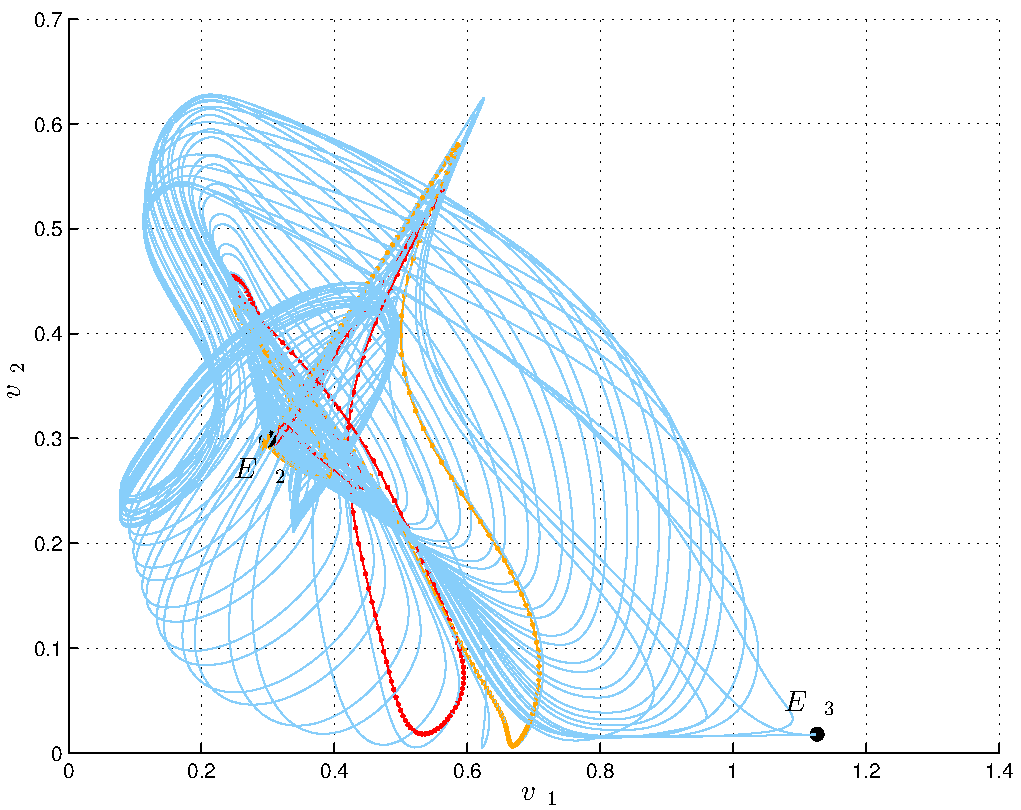
\includegraphics[width=0.35\textwidth]{ks22_E2_manif_homo_rpo_inv}
  (b)~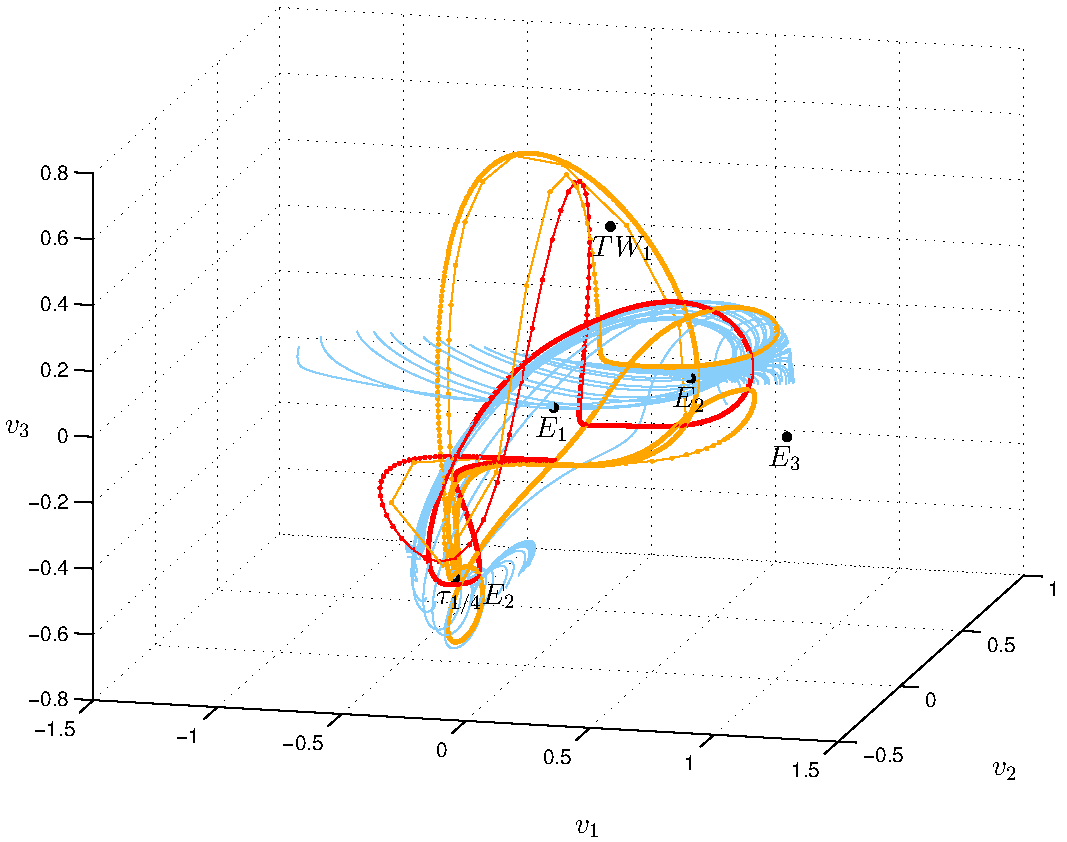
\includegraphics[width=0.35\textwidth]{ks22_E2_manif_homo_rpo_mf1}
  (c)~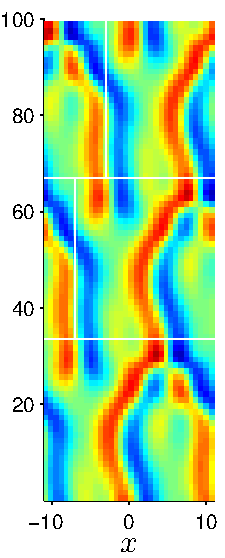
\includegraphics[width=0.09\textwidth, clip=true]{ks22rpo0335-0505}
     ~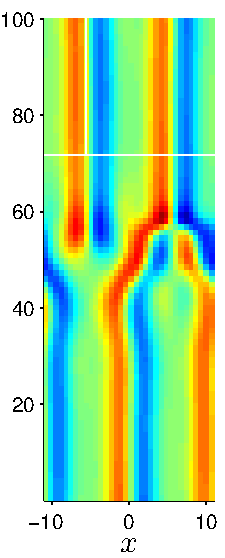
\includegraphics[width=0.09\textwidth, clip=true]{ks22rpo0717-0550}
 \end{center}
  \caption{Unstable manifold of \EQV{2} projected on variables \refeq{eq:SO2polarExt}. The coordinate axes $v_1$,
$v_2$, and $v_3$ are constructed from vectors $\Re\, \jEigvec[1], \Im\, \jEigvec[1]$, and ${\Re\,} \jEigvec[4]$
by Gram-Schmidt orthogonalization (in original space) and transformed to reduced space through transformations
(11) of ksReduced. Two relative periodic orbits with $\period{p} = 33.5$, $\shift_p = 4.04$ (red)
and $\period{p} = 71.7$, $\shift_p = 5.503$ (orange) are also shown. (b) Same as in panel (a) but using a slice with
$c_1=0,\, b_1>0$. (c) Spatial representation of \rpo s with $\period{p} = 33.5$, $\shift_p = 4.04$
and $\period{p} = 71.7$, $\shift_p = 5.503$.
  }
\label{f:ks22_E2_manif_rpo_homo}
\end{figure*}

\begin{figure*}[ht]
 \begin{center}
  (a)~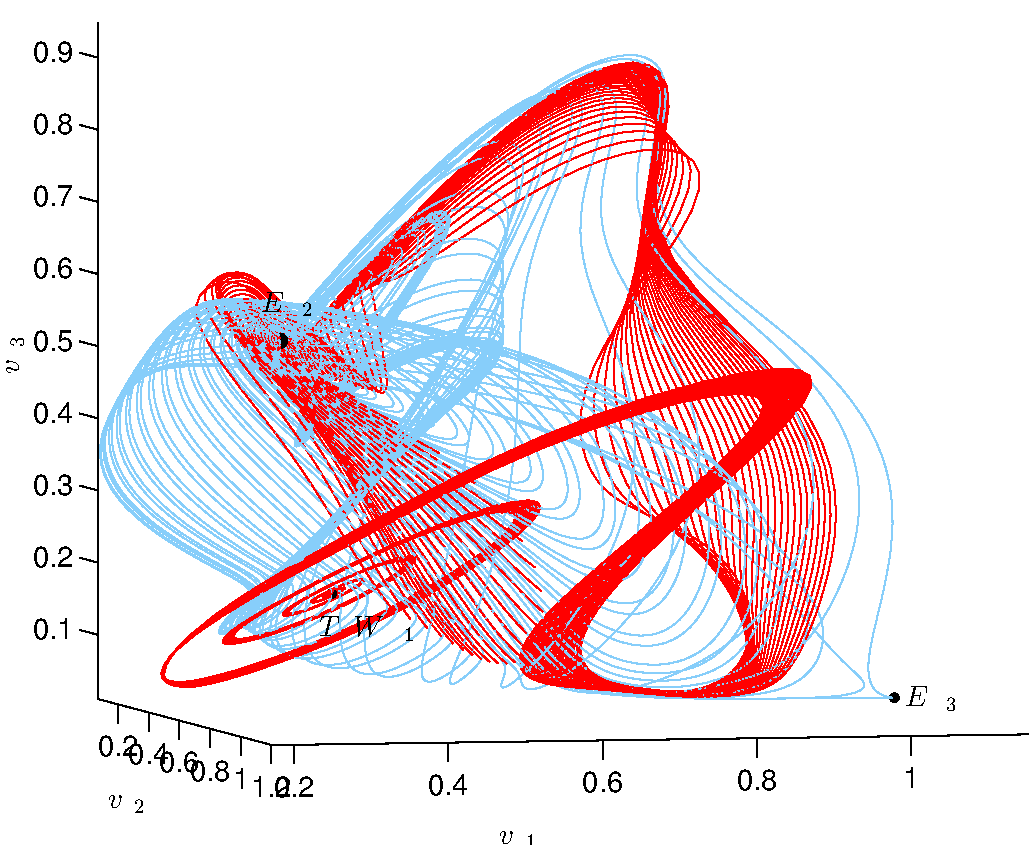
\includegraphics[width=0.45\textwidth]{ks22_TW1_E2_manif_inv}
  (b)~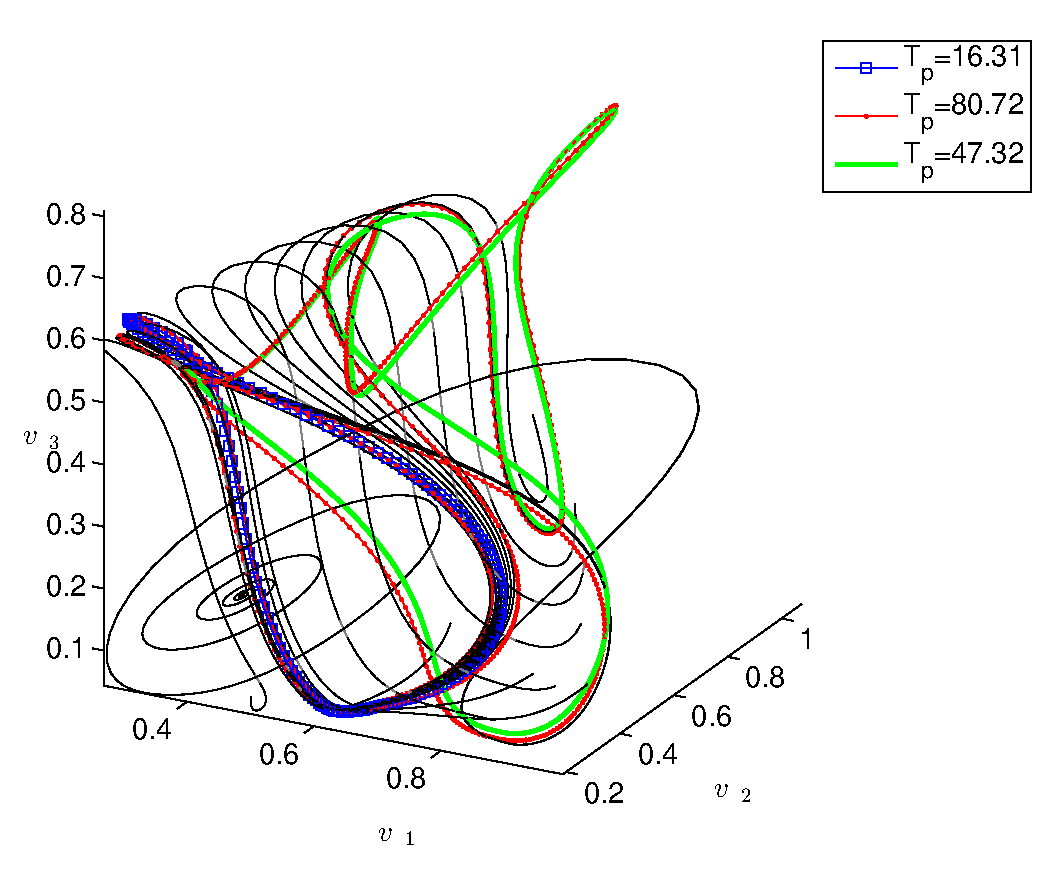
\includegraphics[width=0.45\textwidth]{ks22_TW1_manif_rpos_inv}
 \end{center}
  \caption{Different parts of the unstable submanifold of \REQV{}{1} corresponding to the leading expanding pair of complex eigenvalues
projected on variables \refeq{eq:SO2polarExt}. The coordinate axes $v_1$,
$v_2$, and $v_3$ are constructed from vectors $\Re\, \jEigvec[1], \Im\, \jEigvec[1]$, and ${\Re\,} \jEigvec[3]$
by Gram-Schmidt orthogonalization (in original space) and transformed to reduced space through transformations
\refeq{eq:SO2polarExt}. (a) Trajectories on the unstable manifold of \REQV{}{1} (red) which come to the neighborhood of $\EQV{2}$.
Those which come closest to $\EQV{2}$ leave its neighborhood tracing its unstable manifold (shown in light blue).
(b) Nonlinear folding of trajectories on the unstable manifold of \REQV{}{1} (black) appears related to the existence of
\rpo s of \reffig{f:rpo_shad}. However, it is more efficient to use the manifolds of the shortest orbits to study the corresponding
return maps.
  }
\label{f:ks22_TW1_manifold}
\end{figure*}





\section{Conclusions}

Motivating \refeq{eq:O2inv} is still rough around the edges, but the final result is
1) easily seen to be $\On{2}$-invariant, 2) easily and economically
implemented numerically, requiring no computer algebra, 3) it scales well
with the dimension of phase space, 4) it is global requires no further
thinking of singularities and can thus be used in automated searches for
neighboring orbits in sets of thousands orbits. This is how commencing with the
organization of relative periodic orbits in families, as in \reffig{f:rpo_shad},
became possible.

\appendix

% \section{Alternative basis}
%
% A simple choice is
% \beq\label{eq:SO2polarMag}
%     \tilde{q}_k =
% 		    g_\delta(r_1^2)\,r_k^2\,, \qquad k=2,\ldots,N,
% \eeq
% where $g_\delta(r_1)$ is monotonic, satisfies $g_\delta(0)\neq0$,
% has a convergent Maclaurin series for $0<r_1<\infty$ and
% may depend on a parameter $\delta$.
% % and has to be chosen such that \refeq{eq:SO2polarCont}
% % and \refeq{eq:SO2polarMag} are linearly independent. To fulfill the latter requirement,
% % it is sufficient to choose $g_\delta(r_1)$ such that
% Under these assumptions we can easily show that \refeq{eq:SO2polarMag} and
% \refeq{eq:SO2polarCont} are linearly independent. A simple choice which serves our purposes
% is  $g_\delta(r_1^2)=1$. However, the freedom in choosing more general $g_\delta(r_1^2)$ will be used
% in the following to keep the nonlinear deformation of state-space portraits by the introduction
% of \refeq{eq:SO2polarMag} to a minimum. Eventhough the introduction of
% $N-1$ variables \refeq{eq:SO2polarMag} leads to an apparent increase of state-space dimension,
% we have to note that $\tilde{q}_k$ are not functionally independent from $\tilde{b}_k$
% and $\tilde{c}_k$, since they satisfy $N-1$ relations
% \beq\label{eq:SO2polarSyz}
%   \tilde{q}_k\,h_\epsilon^2(\tilde{b}_1^2+\tilde{c}_1^2) = (\tilde{b}_k^2+\tilde{c}_k^2)\,g_\delta(\tilde{b}_1^2+\tilde{c}_1^2)\,,\quad k=2,\ldots,N.
% \eeq
% Relations \refeq{eq:SO2polarSyz} describe the manner in which the $(2N-1)$-dimensional reduced space is embedded in
% $(3N-2)$-dimensional space of $\tilde{b}_k,\tilde{c}_k,\tilde{q}_k$.
%
% However, even with the introduction of $\tilde{q}_k$ we still fail to span $r_1=0$,
% since points in reduced space are not identified by the $r_k$ alone (\ie\ there are
% $N-1$ variables which depend on appropriate differences of $\theta_k$ missing).
% A strategy towards constructing a complete basis is outlined in the Appendix.
% For the example of \KSe, however, we note that completeness is not essential;
% points with $r_1=0$ in the dynamically important antisymmetric subspace are
% uniquely identified by $q_k$.
%


\bibliography{../bibtex/siminos}

\end{document}
